\section{Experimental Results}\label{sec:exp}
%
In this section, we present our experimental setup and the impact of the different optimizations and implementations described in the previous section.

\mypar{General note about the presented plots}
In all the plots, the red dashed lines in the represent perfect scaling.
For the computation of the speedup on $n$ threads defined as $t_1/t_n$ the mean value of the one-threaded timing $t_1$ of the parallel code was used.

All time measurements were performed using the C++ high precision clock and a list of these single-threaded timings can be found in table \ref{tab:t1timings}.
\par\medskip

  \begin{table}[h]
	  \textbf{Single threaded solution time [sec] for graph size 100k}
    \centering
    \begin{tabular}{lll}
		Implementation	& median & quartile interval \\
    \toprule
	Serial				& $0.150$ & $[0.147,0.151]$ \\
	Node-Lookup			& $0.183$ & $[0.181,0.192]$ \\
	Worksteal			& $0.167$ & $[0.166,0.172]$ \\
	Scatter-Gather		& $0.160$ & $[0.159,0.167]$ \\
    \bottomrule
    \end{tabular}
    %
    \par\medskip
	  \textbf{Single threaded solution time [sec] for graph size 1M}
    \centering
    \begin{tabular}{lll}
		Implementation	& median & quartile interval \\
    \toprule
	Serial				& $2.91$ & $[2.84,2.97]$ \\
	Node-Lookup			& $3.48$ & $[3.40,4.12]$ \\
	Worksteal			& $3.40$ & $[3.33,4.15]$ \\
	Scatter-Gather		& $3.51$ & $[3.01,3.66]$ \\
    \bottomrule
    \end{tabular}
    %
    \par\medskip
    \caption{Median and quartile intervals for single threaded sorting times of a random graph with average node degree 32. The quartile intervals represent the interval between the 25\% and the 75\% percentile.}
    \label{tab:t1timings}
  \end{table}
\par\medskip
The discussion in this paper will focus on the topological sorting of a random graph with average node degree 32.
While the speedup of our implementations highly depend on the graph type (and in particular on its density), the relative positioning of different optimization strategies is consistent between all the graphs that were tested.

%%%%%%%%%%%%%%%%%%%%%%%%%%%%%%%%%%%%%%%%%%%%%%%%%%%%%%%%%%%%%%%%%
% HARDWARE AND COMPILER
%%%%%%%%%%%%%%%%%%%%%%%%%%%%%%%%%%%%%%%%%%%%%%%%%%%%%%%%%%%%%%%%%
\mypar{Hardware and compiler}
The experiments were run on a 24-core system consisting of 2 Intel Xeon E5 processors (see table \ref{tab:hardware}).
Hyperthreading was not used for the benchmarks.
The implementations were written in \Cpp, using OpenMP and GCC atomic built-in functions. The graph was stored in an adjacency list.

  \begin{table}[h]
    \centering
    \begin{tabular}{ll}
    \toprule
    Processor        & Intel Xeon E5-2697 (Ivy bridge) \\
    Max. clock rate  & 3.5 GHz (with TurboBoost)\\
    \# Sockets       & 2 \\
    Cores / socket   & 12 \\
    Threads / socket & 24 \\
    LLC / socket     & 30 MB \\
    \midrule
    Compiler and flags & GCC 4.8.2, -O3\\
    \bottomrule
    \end{tabular}
    \caption{Hardware and compiler used for benchmarks}
    \label{tab:hardware}
  \end{table}
 

%%%%%%%%%%%%%%%%%%%%%%%%%%%%%%%%%%%%%%%%%%%%%%%%%%%%%%%%%%%%%%%%%
% EFFECT OF OPTIMIZATIONS
%%%%%%%%%%%%%%%%%%%%%%%%%%%%%%%%%%%%%%%%%%%%%%%%%%%%%%%%%%%%%%%%%
\mypar{Effect of Optimizations}
To assess the performance gain of the optimizations proposed in the previous section, the Node-Lookup implementation was configured with or without batch-insertion,
and using atomic operations or locks for decrementing the parent counter.
This yields four different configurations, for which their absolute runtimes was measured and is depicted in figure \ref{fig:abstiming}.

Batch-insertion yields a performance gain which is expected since it requires far less locks on the solution list than individual insertion of every node.
However, the performance gain is rather small considering the amount of saved locks.
It might be that the threads do not contend too much even with individual insertion, since inserting a front node only takes a fraction of the time, that a thread needs to process the children of a front node.
In other words, the big bottleneck of the algorithm seems to lie in processing child nodes.

This assumption is further backed by the huge performance gain when using atomic operations instead of locks for the parent counter decrement and check.
Using atomic operations clearly overshadows batch-insertion, i.e. even if batch-insertion is used, the performance gain is only mediocre if atomic operations are not used.

The barrier-free implementation could not be measured in direct comparison, since it could only be implemented for the Scatter-Gather implementation.
However, removing the barriers did not lead to better performance. The reason for this behavior probably lies in the properties of the graphs.
The depth of a graph is logarithmic with respect to the number of nodes. Since the number of barriers is equal to depth, the number of barriers is logarithmic, which can be very, very low compared to the number of nodes.
Hence, the overhead due to barriers is probably negligible.

\begin{figure}[t]
	\centering
	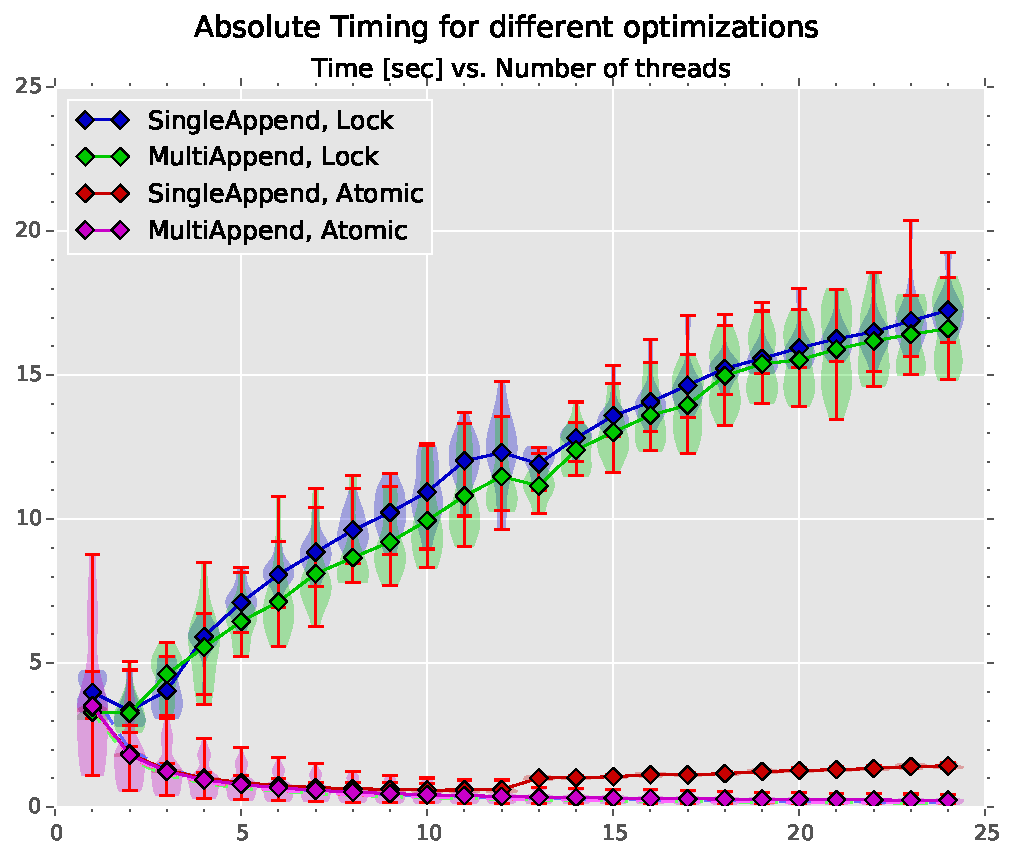
\includegraphics[width=\columnwidth]{plots/abstiming_gtRANDOMLIN_n1000000_deg30.pdf}
	\caption{To compare the effect of different optimizations, the Node-Lookup implementation was benchmarked with batch-insertion turned on or off and with atomic operations or locks for the parent counter.
	As input graph, the random graph with 1M nodes and node degree 30 was used.}
	\label{fig:abstiming}
\end{figure}

%%%%%%%%%%%%%%%%%%%%%%%%%%%%%%%%%%%%%%%%%%%%%%%%%%%%%%%%%%%%%%
% BENCHMARKS
%%%%%%%%%%%%%%%%%%%%%%%%%%%%%%%%%%%%%%%%%%%%%%%%%%%%%%%%%%%%%%

\mypar{Benchmarks of different implementations}
Next the scaling behavior of the optimized implementations is analyzed. All implementations were configured with batch insertion and atomic operations to ensure the best possible performance.
The weak and strong scaling plots are shown in figure \ref{fig:weakscaling} and \ref{fig:strongscaling} respectively.
Both plots confirm a relatively good scaling of both the Workstealing and the Node-Lookup techniques, with the Node-Lookup showing better scaling in both cases.
As for weak scaling, the Node-Lookup implementation is only roughly 3 times slower at sorting a 2400k node graph on 24 threads than it is in the base case. The Worksteal implementation takes approx. 5 times longer than the base case.
There is a relatively high speedup drop between 12 and 13 threads for both weak and strong scaling which can be explained by the hardware on which the program is run. In fact, there are 24 cores but only 12 of them are on the same socket.
%
\begin{figure}[t]
	\centering
	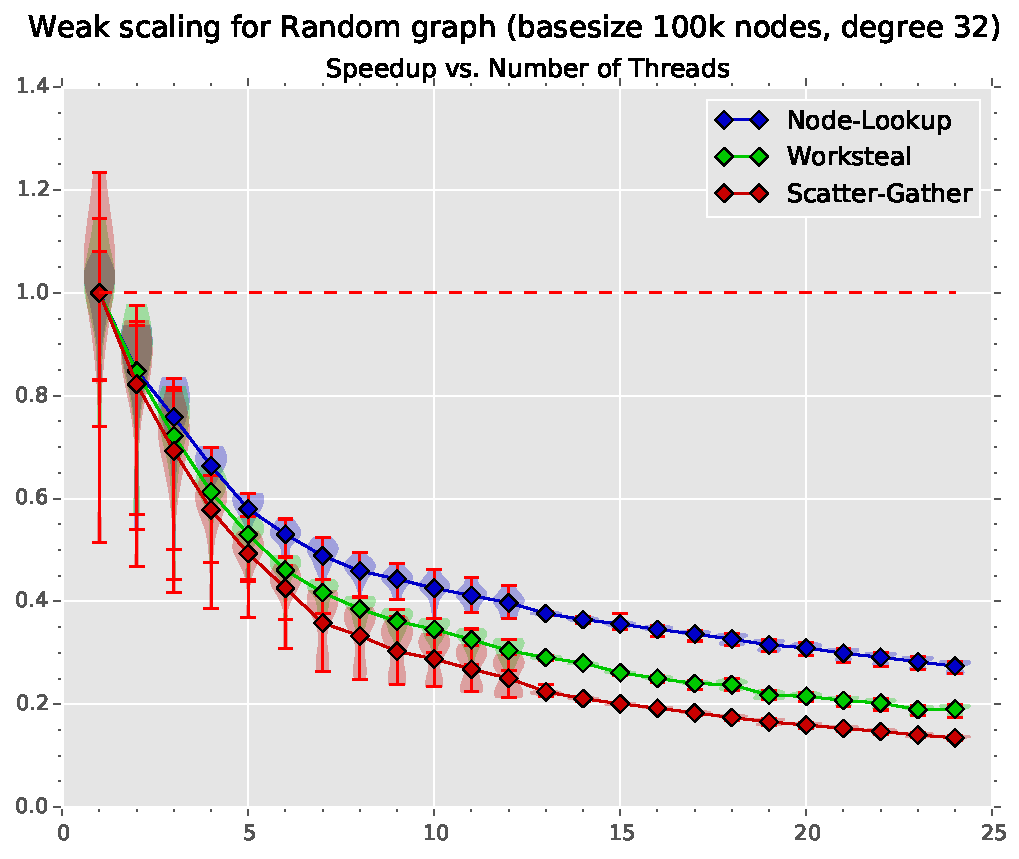
\includegraphics[width=\columnwidth]{plots/weakscaling_gtRANDOMLIN32_n1000000_deg32.pdf}
	\caption{The base size of the graphs in this weak scaling plot is 100k nodes. The effective size in each execution is given by number~of~threads~$\times$~100k
	Absolute timings of the base case with size 100k nodes can be found in table \ref{tab:t1timings}, top
}
	\label{fig:weakscaling}
\end{figure}
%
\begin{figure}[ht]
	\centering
	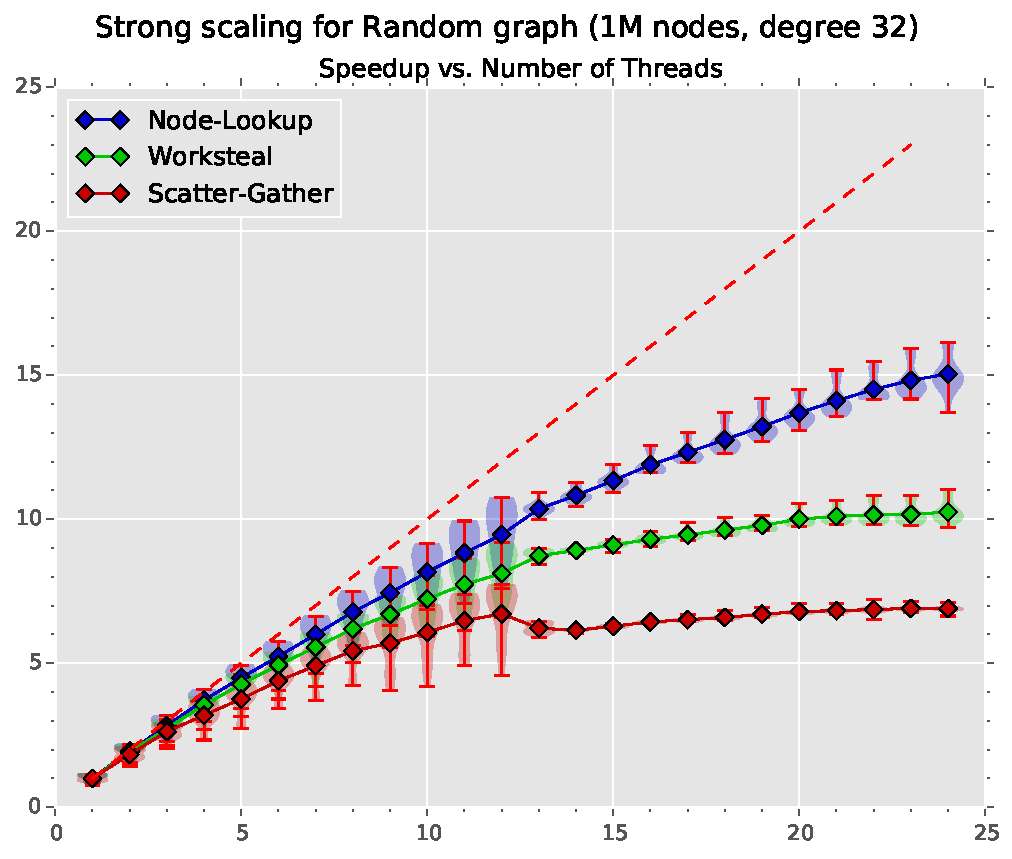
\includegraphics[width=\columnwidth]{plots/strongscaling_gtRANDOMLIN_n1000000_deg32.pdf}
	\caption{The Node-Lookup again shows better scaling than the Worksteal implementation. On 24 cores they achieve a speedup factor of 15x and 10x respectively. (Absolute runtimes can be found in table \ref{tab:t1timings}, bottom)}
	\label{fig:strongscaling}
\end{figure}
%
Bearing in mind the rather serial nature of the topological sorting algorithm, both implementations can be viewed as very successful parallelizations as compared to the simple Scatter-Gather approach.



%%%%%%%%%%%%%%%%%%%%%%%%%%%%%%%%%%%%%%%%%%%%%%%%%%%%%%%%%%%%%%%%%
% GRAPH TYPES
%%%%%%%%%%%%%%%%%%%%%%%%%%%%%%%%%%%%%%%%%%%%%%%%%%%%%%%%%%%%%%%%%
\mypar{Dependency on graph type} So far, our analysis only considered a sparse random graph of average node degree 32.
Next, the performance of parallel topological sorting applied to other graphs is investigated.

For every node, the random graph has $nd$ edges to randomly chosen nodes, where $nd$ denotes the node degree.
A different graph type is the software graph. Its purpose is to model software dependencies. 
As mentioned earlier, resolving software dependencies is one possible application of topological sorting, hence it is considered here.
The construction of this graph was described by \cite{musco2014generative}.

The software graph and the random graph are sparse, i.e. the number of edges $|E|$ is much smaller than the maximum possible number of edges $\tfrac{1}{2}|V|(|V|-1)$.
In particular, the number of edges in the graph scales linearly with the graph size, $|E| \sim \mathcal{O} ( |V| )$).

The influence of the different graphs on strong scaling was measured using Node-Lookup as the reference implementation.
Four different graphs were compared: Three random graphs with node degrees 8, 16 and 32 respectively, and the software graph.
Figure \ref{fig:strongscaling_graphtypes} clearly shows how the scaling behavior improves for graphs with higher density, i.e. more edges per node.
Note that the average node degree in such a software graph is around 2; that is, very low compared to the other graphs.
This means, that the overhead required to synchronize the threads becomes large compared to the work that needs to be performed which in turn destroys a lot of the parallelism.

%
\begin{figure}[ht]
        \centering
        %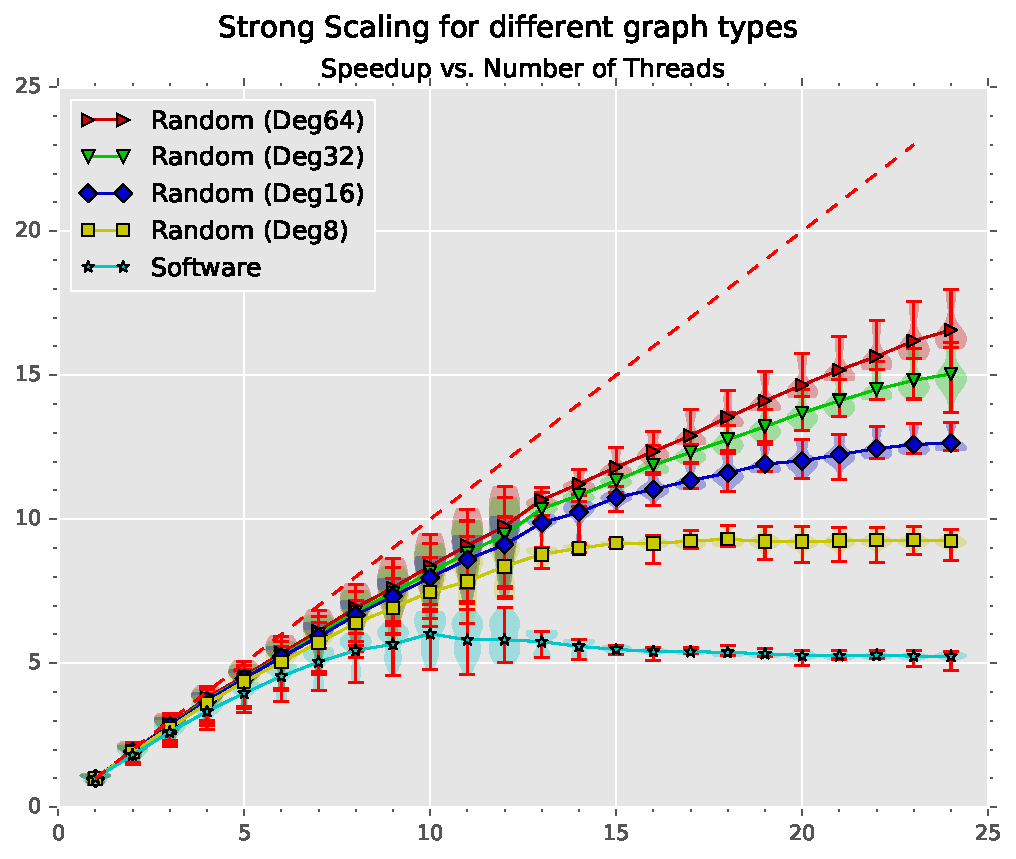
\includegraphics[width=\columnwidth]{plots/strongscaling_gtALL_n1000000.pdf}
        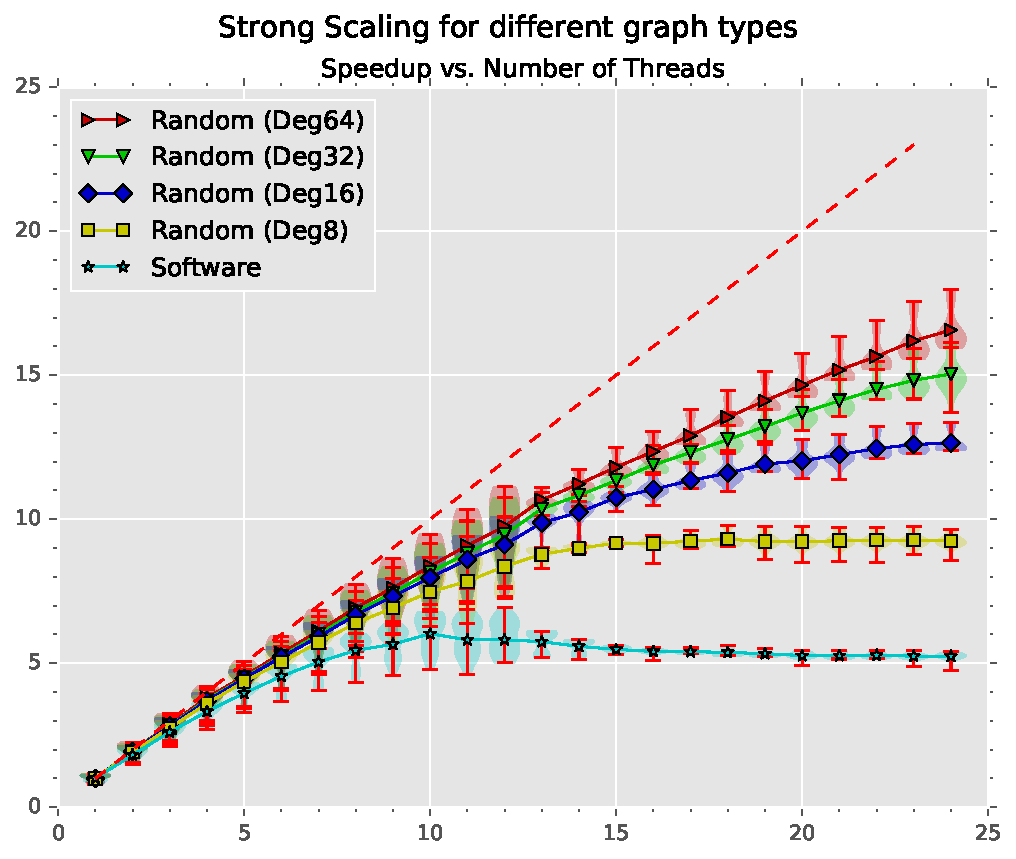
\includegraphics[width=\columnwidth]{plots/strongscaling_gtALL_n1000000_multicolor.pdf}
        \caption{Strong scaling of the Node-Lookup implementation for several different input graphs of size 1M nodes. The scaling is better for random graphs with higher node degree than for those with low node degree.
                The software graph (average node degree approx. 2) achieves a speedup of roughly 6x on 10 threads but does not scale any further.
}
        \label{fig:strongscaling_graphtypes}
\end{figure}
%

Although all tested graphs are artificial (i.e. they do not come from real-world datasets but are rather constructed to meet some requirements),
the fact that scaling strongly depends on a graph's node degree can be expected for real-world graphs as well.
The actual performance of our implementations on such graphs was not tested and an investigation of such could be content of further research.